%We now evaluate the potential for prediction of HS using the Traumabase. For that, we perform a prediction with CV (cf Chapter \ref{validation}) and compare it with other methods of HS evaluation. An advantage of imputation is that one can predict with various models: we compare predictions using logistic regression \cite{hosmer2013logreg}, Support Vector Machines (SVM) \cite{hearst1998SVM} and random forests \cite{svetnik2003RF} in predicting the probability of HS.

Our final step is to see how well prediction with imputation works to predict hemorrhagic shock. For that, we proceed to cross-validation (cf Chapter \ref{validation}) to get an idea of the performance we can achieve this way. We compare it to several references to see whether this is an improvement over other methods of prediction.
	\section{Methodology}
		\subsection{Prediction pipeline}
To evaluate our method we perform imputation and prediction on the data, by training on a training set $X_A, y_A$ and validating on $X_V, y_V$. In order to get an idea of the average performance, we repeat this for multiple $X_A, X_V$ splits.

An interest of imputation is that once missing data is imputed, any full-data method can be used for prediction. To illustrate this, after imputation we perform prediction using three different methods: logistic regression \cite{hosmer2013logreg}, Support Vector Machine (SVM) \cite{hearst1998SVM} and random forest (RF) \cite{svetnik2003RF}. 

		\subsection{Evaluating the prediction}
\paragraph{Metric}
The response variable in our data is binary, and we predict a probability. This, and the unbalance in the response (only 10\% of positive cases) means that the choice of metric is not straightforward. A first choice we have to make is whether we choose a threshold for the prediction (predict a positive when the predicted probability is above some value), or evaluate the predicted probability as-is.

Some metrics allow us to evaluate the predicted probability directly, such as the AUC \cite{huang2005AUC} or log-loss (minimized by the logistic regression). However, we want to be able to compare our results with those given by scores or the historical decisions of doctors, which are binary. We want to see if our predictions are able to separate patients with and without shocks at least as well as those references, so we need a metric that puts our predictions and those scores on an equal footing.

To that end, we choose a simple cost function that, given a binary prediction, assigns some user-defined cost to false negatives and false positives. That is:

$$ L(\hat{y}, y)=\frac{1}{n} \sum \limits_{i=1}^n c_1 \mathbb{1}_{y_i=1,\hat{y}_i=0} + c_2 \mathbb{1}_{y_i=0,\hat{y}_i=1}$$

with $c_1 + c_2 = 1$.

To evaluate our predicted probability, we take the best value of this loss for any choice of threshold: this gives us a measure of the separation power of those predictions. The choice of costs is not obvious, which is why in this chapter we show the results for multiple possible values.

\paragraph{Comparison}
In order to have a reference performance for HS prediction, we compare the value of the loss with the loss obtained from several other predictions:
\begin{itemize}
\item \emph{Doctor's prediction:} The decision to initiate a MT procedure is recorded in the Traumabase. It determines whether the doctor considered the patient to be at risk of HS.
\item \emph{ABC (Assessment of Blood Consumption)\cite{nunez2009ABC} score:} this gravity score is the only one that was designed with prehospital prediction in mind. It is a very simple score that only uses a few measurements.
\item \emph{TASH (Trauma Associated Severe Hemorrhage)\cite{yucel2006tash}) score:} this score was also designed for hemorrhage detection, but at a later stage: it uses some values that are only available after laboratory tests (e.g. base excess) or radiography (presence of a fracture).
\item \emph{SAEM Logistic regression:} this a method for logistic regression without imputation of the training dataset, developed by Jiang \cite{jiangsaem} to address the specific issue of HS prediction on the Traumabase. If we take the notations from Chapter \ref{validation}, the idea is that $\alpha$ the imputation parameter and $\beta$ the regression parameter are learned jointly rather than one after the other. 
\end{itemize}

This gives us some points of comparison for predictive performance.

		\subsection{Choice of imputation method}
There are many methods of imputation we can choose from (cf Chapter \ref{imputation}) to impute missing values in. In order to compare them, we proceed to grouped imputation (as described in Chapter \ref{validation}) with each of them, and then perform a prediction on each imputed dataset. The resulting validation errors are presented in figure \ref{fig.imp_method}.

%\begin{figure}[h]
	\centering
   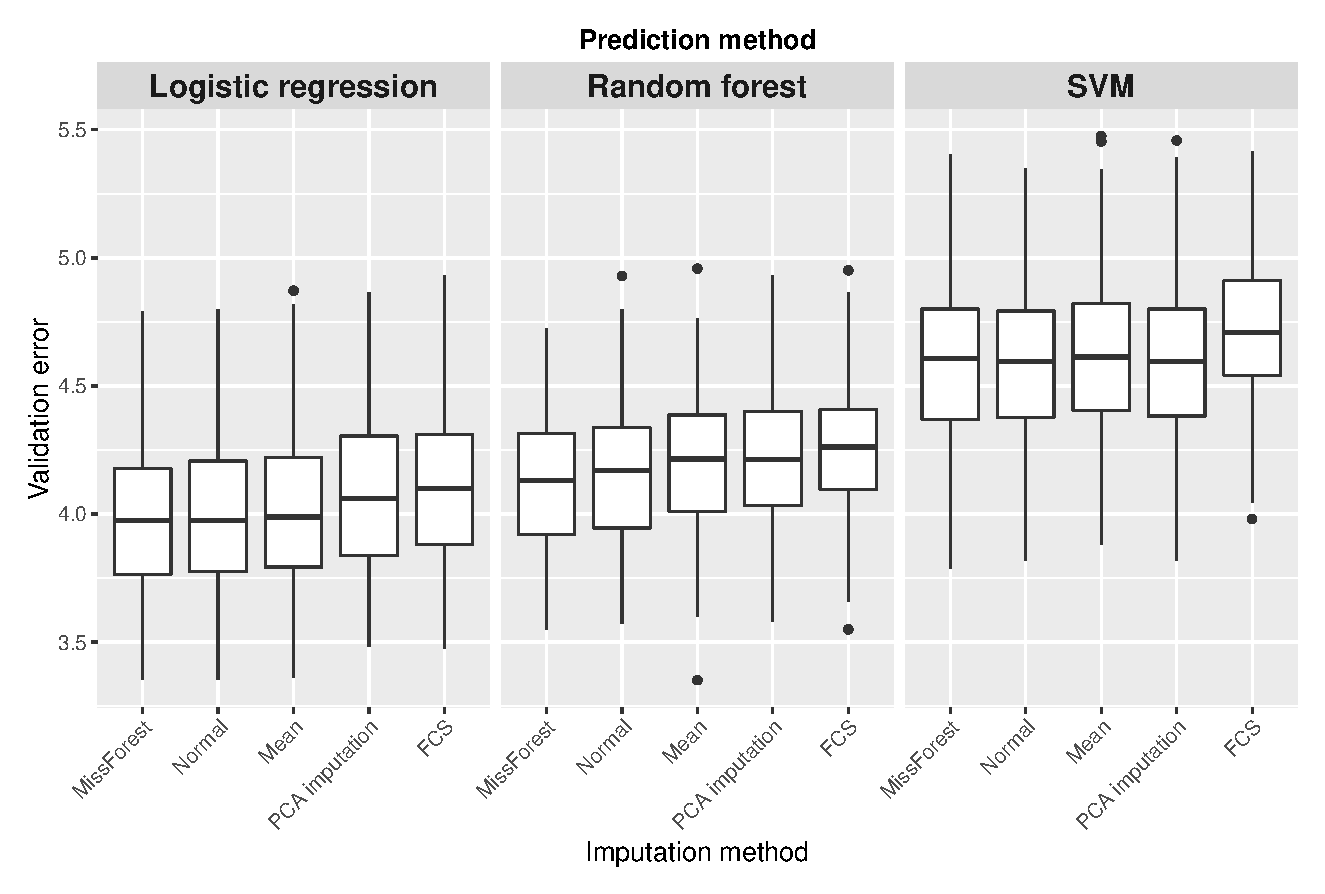
\includegraphics[scale=0.6]{Resources/imp_method}
   \caption{Prediction performance for multiple prediction and imputation methods}
   \label{fig.imp_method}
\end{figure}

It is striking that the difference between imputation methods is very small: even though there are differences in the mean performance, these differences are manor compared to the variation of the performance for different CV splits.

	\section{Results}
We performed predictions on the Traumabase data as described above, for 16 different CV splits. Figure \ref{fig.final_pred} shows the average loss of each prediction (ours and the reference values) for different values of $\frac{c_1}{c_2}$. 

%\begin{figure}[h]
	\centering
   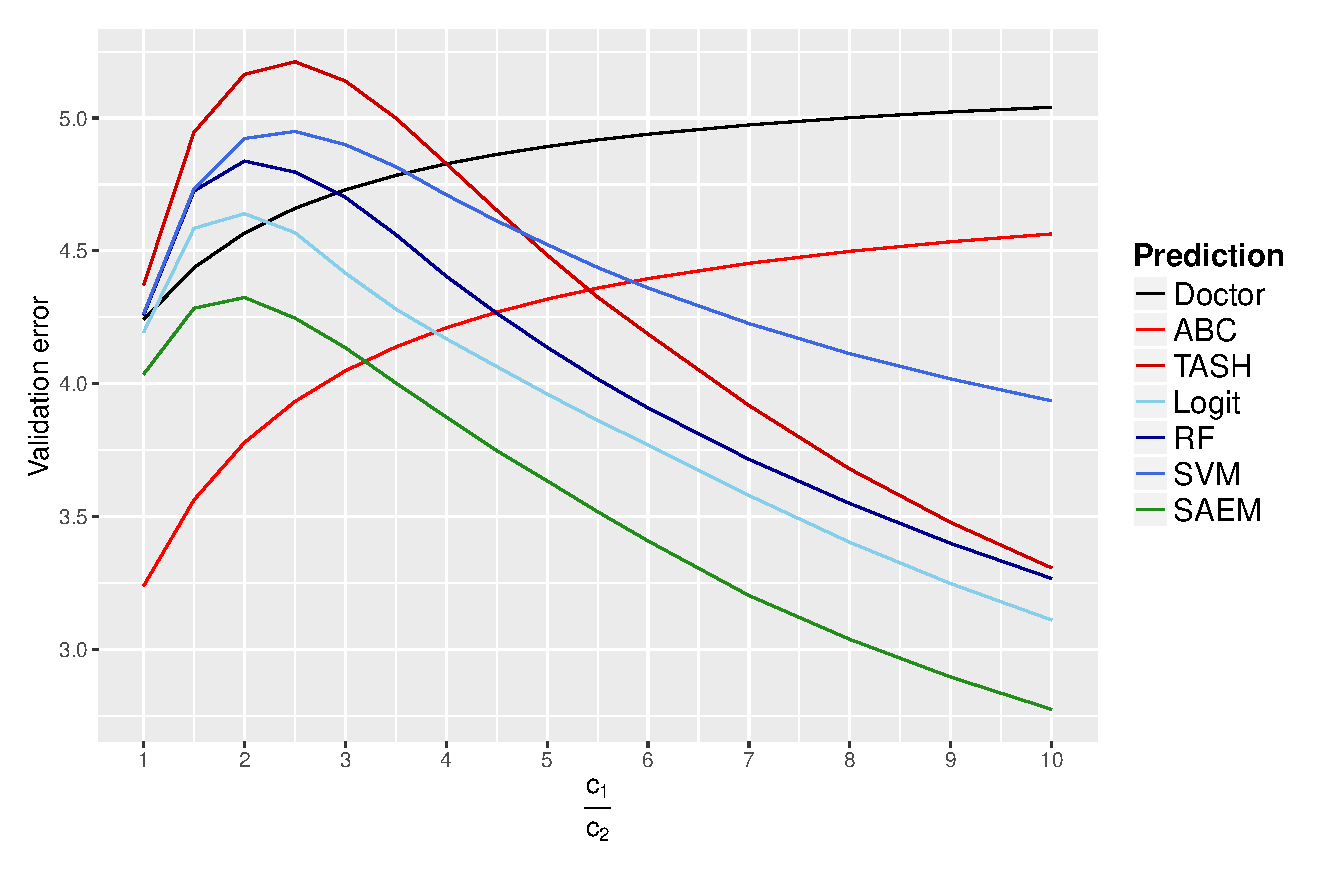
\includegraphics[scale=0.6]{Resources/final_pred}
   \caption{Error for each prediction depending on $c_1, c_2$}
   \label{fig.final_pred}
\end{figure}

First note that there are two possible main trends for the loss depending on the method:
\item The loss increases with $c_1$: this means that the predictions are more conservative, and tend to have fewer false positives but more false negatives. This is the case of the doctors' prediction and the ABC score.
\item The loss decreases when $c_1$ increases: this means that the prediction tends to favor overpredicting HS, so it has fewer false negatives but more false positives. This is the case of all our predictions, as well as the TASH score and SAEM prediction.

When two predictions follow the same trend, it is easy to compare them as one is usually above the other regardless of the choice of weights. In particular, the ABC score seems to be strictly better at predicing hemorrhage than doctors, even though it is extremely simple in principle.

Likewise, we see that for the descending trend, the best predictor is without a doubt the SAEM regression, followed by the logistic regression with imputation, the random forest with imputation, the TASH score and the SVM with imputation in that order.

Whether the ABC score should be preferred to other predictors depends on the choice of weights: for the SAEM prediction, the loss is lower than for ABC if $\frac{c_1}{c_2}$ is greater than approximately 3, while for the regression with imputation this happens for a ratio above 4.

All in all, what this shows is that although imputation gives promising results, for a given model there is a tangible advantage to performing a joint prediction rather than separating imputation and prediction. 

Still, imputing is a good first step: thanks to grouped imputation and subsequent prediction, we can evaluate a method's promise using only out-of-the box methods, without having to create a dedicated model. For instance, we can see that it is visibly not worth trying to implement a model for SVM with missing data. If for instance the performance on the imputed data had been better for RF than for logistic regression, it would have given us a strong case for building a missing-data random forest as a next step. Model selection using imputed datasets allows us to single out one method that we can then choose to improve by implementing it to work without imputation. 